\begin{voorstel}{Waterstof}
\meeschrijver{Mark Leenen}

\begin{samenvatting}
We zijn in 2030 overgestapt van de huidige fossiele brandstoffen economie naar een groene waterstof economie. Waterstof wordt overal toegepast waar geen duurzamere of efficiëntere andere decarbonisatie mogelijk was. De overgang naar de waterstofeconomie heeft Nederland veel banen opgeleverd en een wereldwijde koppositie in waterstoftechnologie.
\end{samenvatting}

\begin{uitdaging}
Waterstof is een gas dat gebruikt kan worden als opslagmiddel voor energie (electriciteit), of als brandstof voor industriële processen op hoge temperatuur, of als grondstof voor de (chemische) industrie. Via brandstofcellen kan waterstof omgezet worden in electriciteit, bijvoorbeeld voor de aandrijving van electromotoren in de transportsector. Waterstof is in deze tijd zo’n interessant gas, omdat het geen koolstof bevat zoals fossiele brandstoffen of aardgas. Gebruik van waterstof voor verschillende doeleinden is daarom vrij van emissie van CO2, en zo een essentiële bouwsteen van een klimaat-neutrale wereld.

Waterstof wordt momenteel vooral gemaakt uit koolwaterstoffen zoals aardgas. Bij die processen komt CO2 vrij. Deze klassiek gemaakte waterstof wordt grijze waterstof genoemd. De vrijgekomen CO2 kan ondergronds opgeslagen worden, waardoor CO2 uitstoot bespaard wordt. In dat geval wordt gesproken van blauwe waterstof. Grijze en blauwe waterstof passen beiden niet in een klimaatneutrale toekomstvisie. Grijze waterstof is volledig buiten scope van dit voorstel. 

Waterstof is ook te maken zonder CO2 uitstoot, met water als grondstof en zuurstof als bijproduct. Dit zogenoemde electrolyseproces levert “groene” waterstof op. De electriciteit die gebruikt wordt voor deze electrolyse is in het beste geval uit een hernieuwbare bron; groene waterstof wordt meestal in 1 adem genoemd met grote windmolenparken op zee.

Nederland is momenteel na Duitsland al de grootste producent van waterstof in Europa, met een productie van 8 miljard m3 per jaar. Deze (grijze) waterstof is vooral bedoeld als grondstof voor de chemische industrie, en zal de transitie moeten maken via blauw, naar groen (bij schaalgrootte die de kostprijs van groene waterstof rechtvaardigt). Alle infrastructuur die geschikt is voor grijze of blauwe waterstof, blijft geschikt voor groene waterstof.

Groene waterstof is alleen rendabel bij voldoende schaalgrootte. Die schaalgrootte kan alleen ontstaan bij voldoende vraag. Vraag en aanbod moeten samen gestimuleerd worden om de waterstofeconomie van de grond te krijgen.

Waterstofgas heeft andere eigenschappen dan aardgas (methaan). Technische uitdagingen zitten in het geschikt maken van delen van het aardgasleidingnetwerk voor waterstof. En in de toepassing van waterstof als brandstof in hoog-temperatuur processen in de industrie. 
\end{uitdaging}

\begin{overwegingen}

\includegraphics[width=.5\textwidth]{img/energie/waterstof-tank}

Waterstof is een energie-opslag medium. Het proces van energie-opslag in waterstof leidt tot energieverlies (-25\%), en het vrijmaken van energie uit waterstof kost wederom energie (-40\% van het restant). Qua energie-efficientie scoort waterstof geen hoge ogen. Daarom zal waterstof alleen een rol spelen in decarbonisatie van processen en sectoren waar decarbonisatie op andere manieren (zoals directe elektrificering) niet mogelijk is. Desondanks zal waterstof een zeer belangrijke en omvangrijke rol spelen in klimaatneutraliteit!

Nederland is goed gepositioneerd om een leider te worden in de waterstofeconomie. De Noordzee biedt gelegenheid voor grote windparken, waarvan de duurzame elektriciteit gebruikt kan worden voor electrolyse van (demi-)water tot groene waterstof. Nederland heeft een bestaande gas-infrastructuur die deels geschikt gemaakt kan worden voor waterstof [Gasunie]. En Nederland heeft een sterke logistieke en chemische sector, waar waterstof goed in zal passen. Daarnaast heeft Nederland grote lege gasvelden, waar CO2 in opgeslagen kan worden vanuit de productie van blauwe waterstof.

Gedurende de jaargetijden waarin zonnepanelen veel energie opwekken, en in tijden van veel wind(energie), kan het overschot opgeslagen worden in de vorm van waterstof. In de maanden waarin weinig zonne-energie opgewekt wordt, of wanneer het minder waait, wordt het tekort dan aangevuld vanuit waterstof of zoet-zout water batterijen (al staan die nog in de kinderschoenen).

In de logistiek is zwaar transport (waar Li-ion of solid state batterijen niet meer toepasbaar zijn vanwege te trage laadsnelheid of te lage mogelijke capaciteit) zoals internationaal vrachtverkeer over de weg de sweet spot voor waterstof. Deze sector heeft zich verenigd in de European Clean Trucking Alliance (ECTA). Al vanaf 2021 kan de Total Cost of Ownership van een vrachtwagen die rijdt op waterstof, concurreren met diesel. Vanaf 2021 kan ook langzaam accijns geheven worden op waterstof, om de investeringen in de waterstofeconomie terug te gaan verdienen. [W2H2] Vrachtwagens op basis van brandstofcel kunnen mede door Nederlandse bedrijven ontwikkeld en gebouwd worden (DAF en Scania, Holthausen Clean Technology). 

De lancering van de European Clean Hydrogen Alliance (ECH2A) op 8 juli 2020 laat zien dat Europa vol op waterstof in wil zetten. In Hydrogen Europe is de complete productieketen voor waterstof vertegenwoordigd door 160+ bedrijven, inclusief Nederlandse spelers. Ook lopen er al projecten om groene waterstof van en naar Nederland te transporteren (Green Spider, Green Flamingo \& H2Go, hydrogen4climateaction.eu).

Voor het vliegverkeer komt 2030 te vroeg, en zal het nog steeds kerosine zijn dat de klok slaat. Ook scheepvaart op groene waterstof is in 2030 nog niet op grote schaal mogelijk; hier zal nog diesel, dan wel compressed/liquefied natural gas (CNG/LNG) gebruikt worden. Al wordt toepassing in de scheepvaart wel al onderzocht in het Blue Dolphin project. [Hydrogen4climateaction.eu] Visie is wel dat zowel luchtvaart als ook scheepvaart waterstof als brandstof kunnen gaan gebruiken!

In de industrie zal waterstof een rol spelen als brandstof voor industriële processen die een temperatuur > 250 C nodig hebben [Quintel]. Die processen zijn namelijk moeilijk direct te electrificeren. Momenteel wordt waterstof al bijgemengd bij methaan voor zulke processen. Ook kan waterstof op termijn biomassa vervangen als brandstof, waardoor dat een tijdelijke energiebron zal zijn. Waterstof kan ook in plaats van methaan als grondstof dienen voor productie van kunstmest (ammoniak), en toepassing in of synergie met de staalindustrie biedt eveneens mogelijkheden tot decarbonisatie.

Het huidige gasnet wordt aangepast en uitgebreid, zodat het in 2030 ook deels gebruikt kan worden voor transport van waterstof. Die waterstof is echter vrijwel niet bestemd voor huishoudens, maar grotendeels voor de industrie en transport! In de gebouwde omgeving is een zo klein mogelijke rol voorzien voor waterstof. Hier blijft “gasvrij” het credo, tenzij dat niet kan en een CV ketel op waterstof de beste oplossing blijkt (zoals voor oudere woningen die niet op een warmtepomp over kunnen vanwege slechte isolatie). Transport van waterstof over land zoveel mogelijk via pijpleidingen (niet via trucks). Voor afstanden < 1000 km is de efficiëntie van transport van waterstof door pijpleidingen zeer goed (>95\%). [BOSSEL]

Een windpark op zee kan zowel de opgewekte elektriciteit direct aan land brengen, als ook op zee electrolyzers aandrijven om waterstof te maken (en die aan land te brengen via een gasnet). Beide opties zijn in overweging. Voordelen van electrolyse op zee is dat er geen buffering nodig is voor de variabele electriciteits-levering van een windpark. In het verlengde daarvan kan transport van waterstofgas, boven transport van electriciteit, een kostprijsvoordeel opleveren [hy-gro].
\end{overwegingen}

\begin{aanbevelingen}
De windparken op zee moeten in de toekomst een mix van elektriciteit en groene waterstof (middels electrolysers op zee) leveren. De ratio tussen elektriciteit en groene waterstof moet nader bepaald worden.

Er moet een landelijk waterstof pijpleiding netwerk gerealiseerd worden waarop alle grote afnemers (industrie, transport) aangesloten worden. Het bestaande gasnet kan hier voor een belangrijk deel als basis voor dienen. 

Particulier, lokaal (incl tractoren en licht vervoer in busjes) en streekvervoer maakt in beginsel geen gebruik van waterstof als energiedrager, maar rijdt op batterijen. In deze segmenten is een gedragsverandering (tot een half uur snelladen onderweg, of overnacht laden op bestemming) goed mogelijk. Voor decarbonisatie van dieseltreinvervoer op trajecten die nu geen bovenleiding hebben, kan waterstof of alsnog voor de aanleg van bovenleidingen gekozen worden.

Zwaar transport (vrachtvervoer) moet overstappen op waterstof als brandstof, met toegewijde waterstoftankstations langs snelwegen, die aangesloten zijn aan het waterstof gasnet. Dit geheel moet van de grond komen als 1 megaproject, omdat alle onderdelen van deze keten (vraag en aanbod) elkaar nodig hebben om de pilotschaal te ontgroeien. Voor inclusie van internationaal transport is het onontbeerlijk om de waterstofeconomie op Europees niveau te ontwikkelen. 

Voor gebruik als brandstof in hoog-temperatuur processen in de industrie, is blauwe waterstof zuiver genoeg, en goedkoper: daarom een geschikte (tussen)oplossing. Die blauwe waterstof kan lokaal geproduceerd worden. De bijbehorende CO2 opslag moet uitgewerkt worden (locatie en hoeveelheid). Deze industriële locaties moeten wel al aangesloten worden op het groene waterstof net, en overstappen op groene waterstof wanneer dit kan (kostenverlaging van groene waterstof door schaalgrootte; geen opslagmogelijkheid meer voor CO2). In de loop van de komende decade kan groene waterstof al bijgemengd worden bij blauwe of grijze waterstof, om vraag voor groene waterstof te creëren.

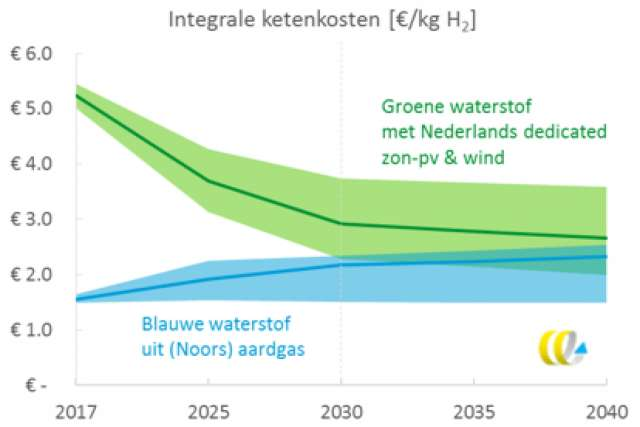
\includegraphics[width=.5\textwidth]{img/energie/waterstof-ketenkosten}

\end{aanbevelingen}

\paragraph{Literatuur}
http://hydrogeneurope.eu

http://hy-gro.net

Wind-to-hydrogen (W2H2) TKI Systeemintegratie Studie TES1216101

https://www.flightglobal.com/air-transport/forget-batteries-is-hydrogen-the-holy-grail-for-carbon-free-commercial-aviation/139150.article

\url{https://www.nrc.nl/nieuws/2020/07/08/brussel-omarmt-waterstof-a4005372#/handelsblad/2020/07/09/#301}

Ulf Bossel, “Does a hydrogen economy make sense?”, Proceedings of the IEEE, Vol. 94, No. 10, 2006, 1826 - 1837

J. Reijerkerk and G. van Rhee, “Waterstof: kansen voor de Nederlandse industrie”, Oktober 2019

https://clean-trucking.eu/publications/europes-opportunity-to-decarbonise-the-road-freight-sector/

http://www.hydrogen4climateaction.eu

Commissie Economische Zaken en Klimaat, “Kabinetsvisie Waterstof en Routekaart Groen Gas: Position Papers Reader”, 7 mei 2020

Institute for Sustainable Process Technology, “Hychain 1,2 \& 3: Energy carriers and hydrogen supply chain”, december 2019

https://www.portofrotterdam.com/nl/havenkrant/havenkrant-43/grootste-groene-waterstoffabriek-van-europa

https://www.natuurenmilieu.nl/themas/energie/projecten-energie/waterstof/waterstof-de-waterstofladder/


\end{voorstel}
